\section{Compléter la figure (5 points)}

\begin{multicols}{2}
	\begin{questions}
		\question[1] Construire la figure ci-contre.
		\question[2] Construire le symétrique de ce quadrilatère par rapport à la droite $(BC)$. Noter $A'$ et $D'$ les symétriques de $A$ et $D$. Les traits de constructions doivent rester visibles.
		\question[2] On note $O$ le milieu du segment $[DD']$. Compléter la figure pour que $O$ soit le centre de symétrie de la figure. Les traits de constructions doivent rester visibles.


	\begin{center}
		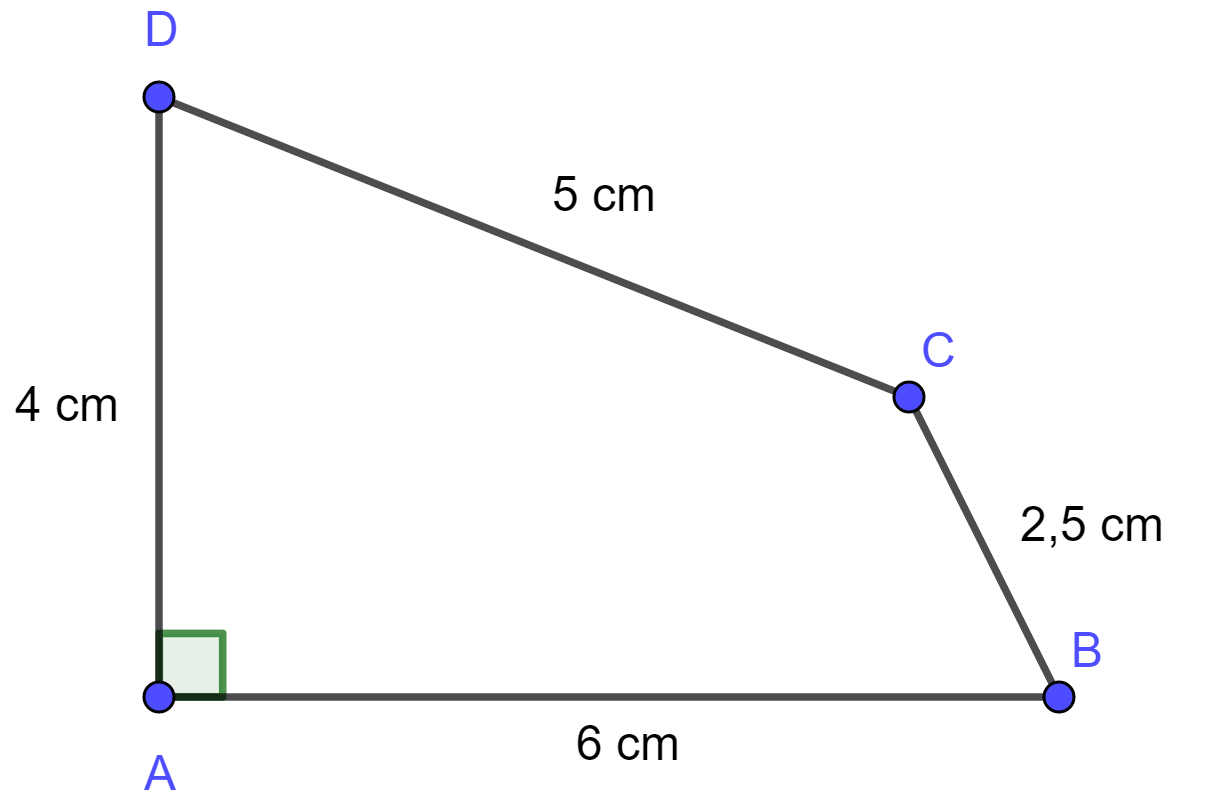
\includegraphics[scale=0.25]{img/cons}
	\end{center}

	\begin{solution}
		\begin{center}
			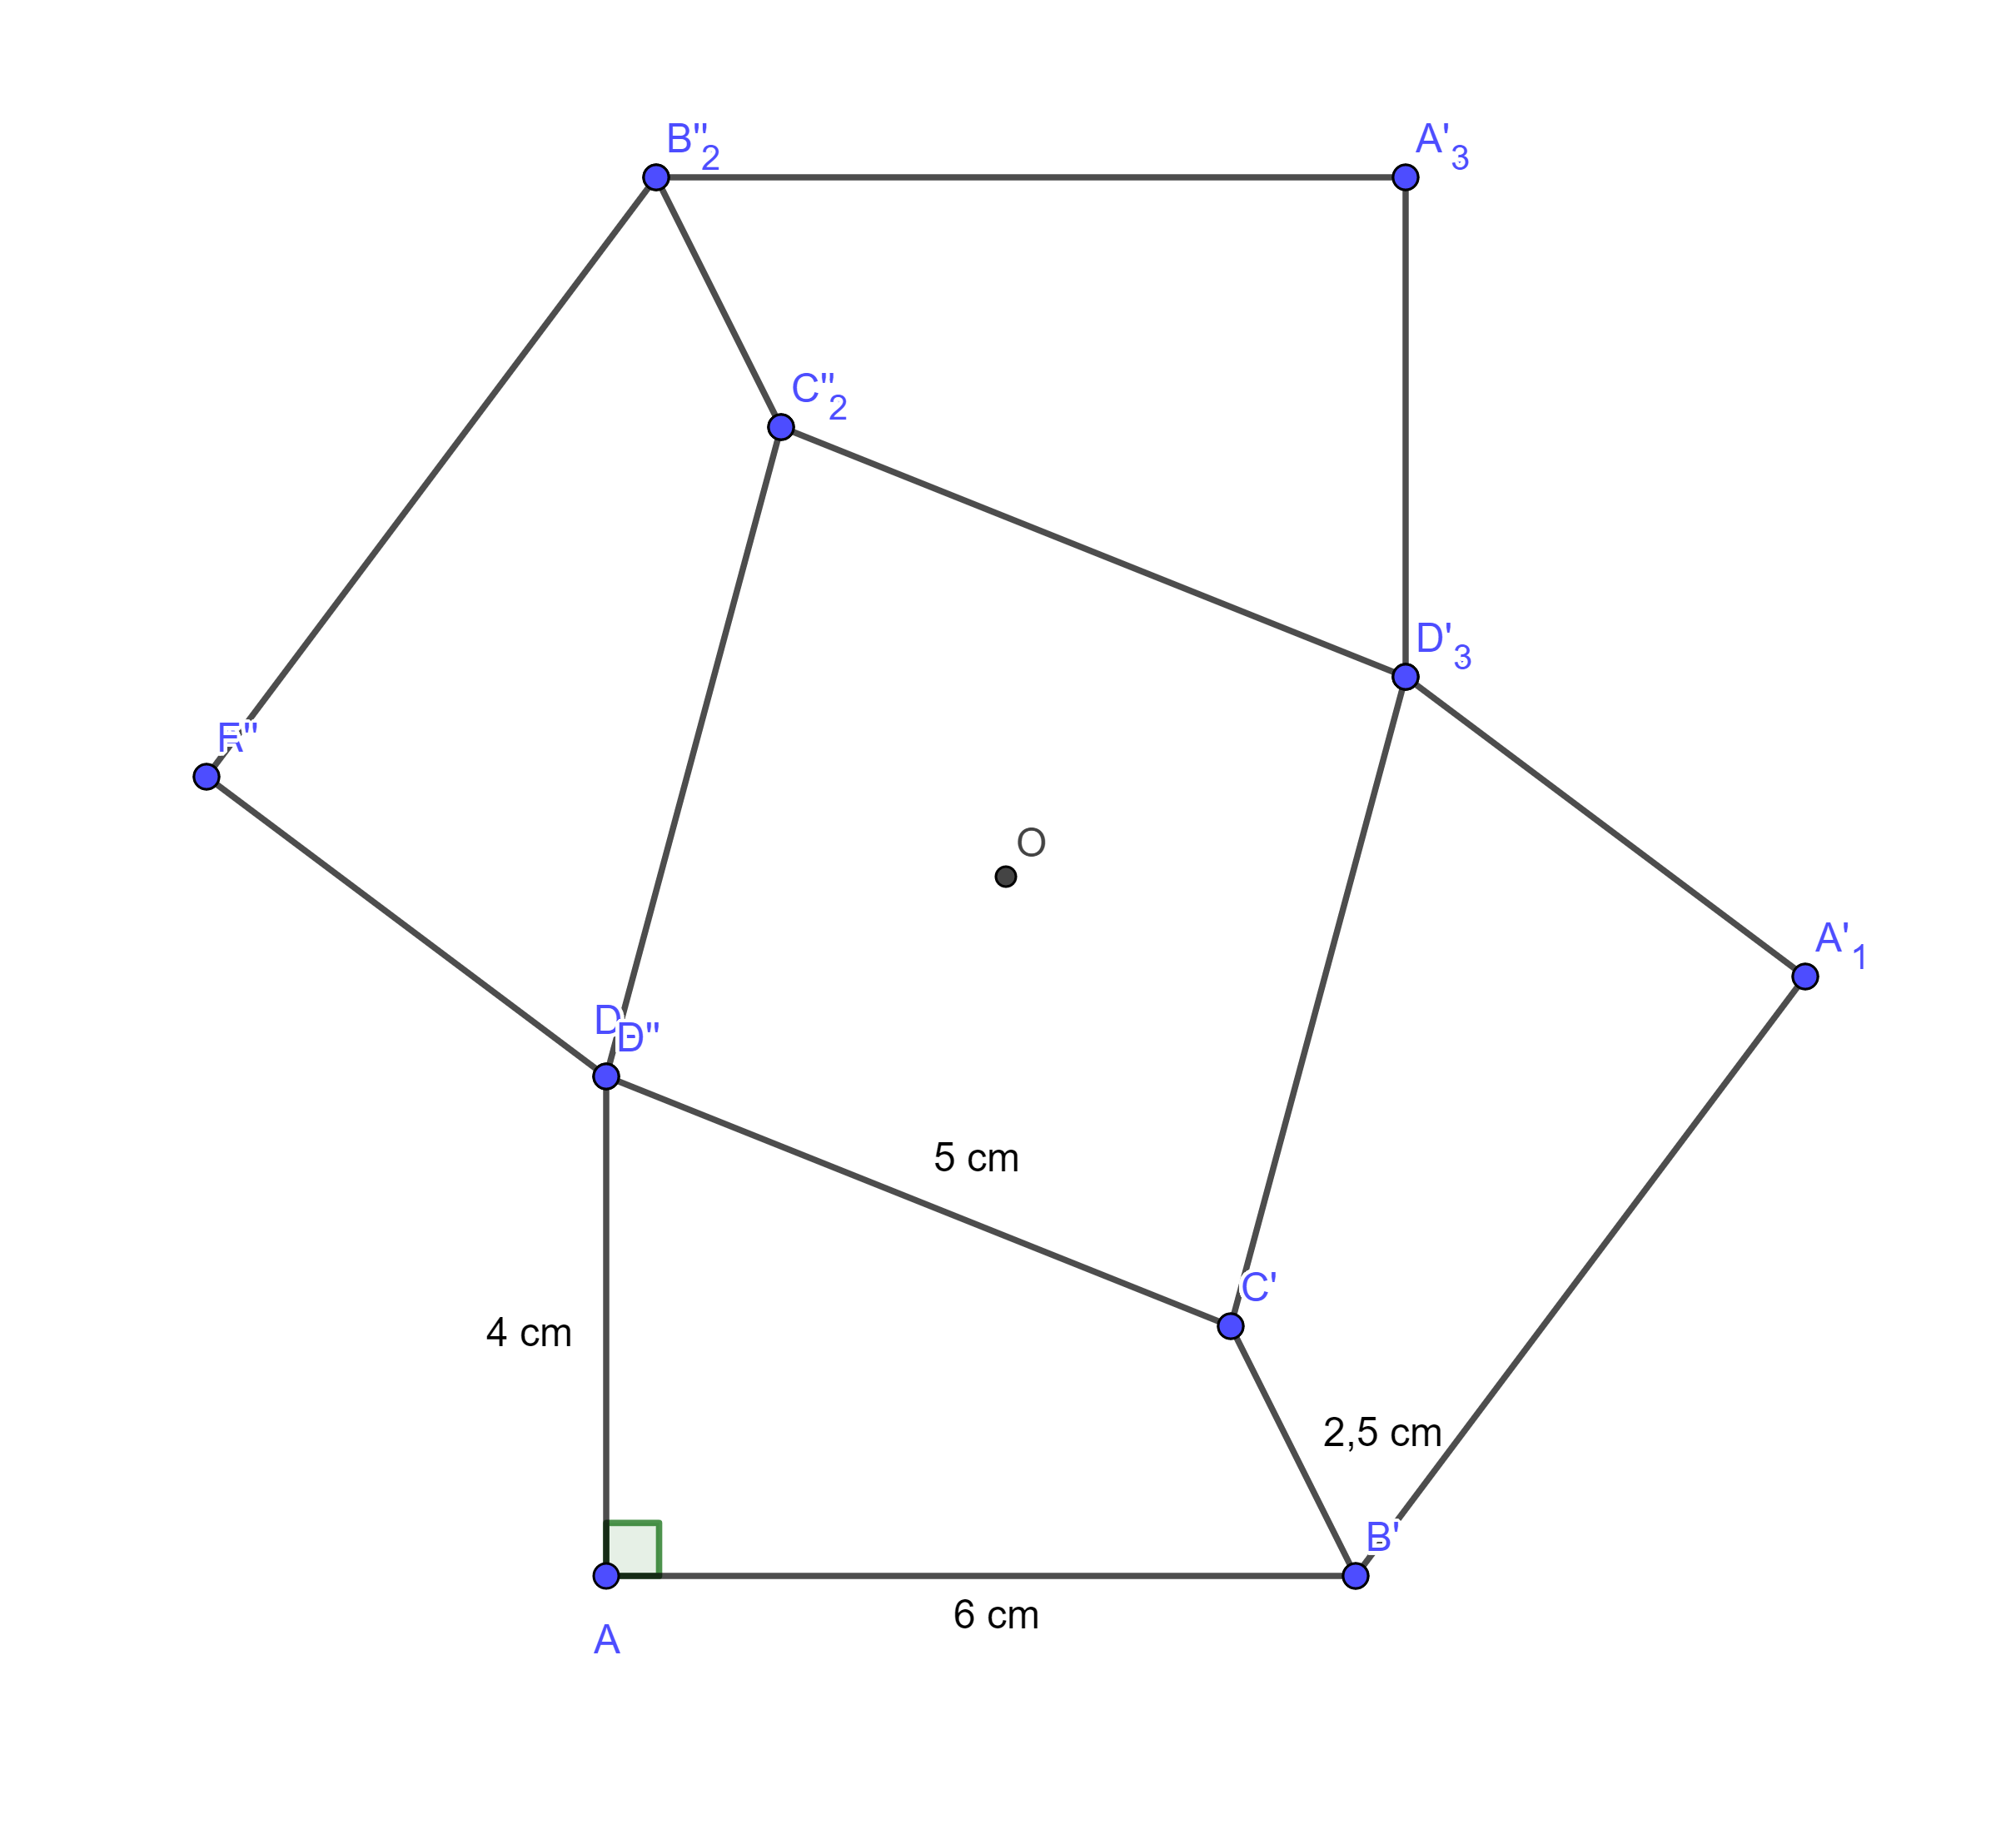
\includegraphics[scale=0.15]{img/cons_corr}
		\end{center}		
	\end{solution}

	\end{questions}
\end{multicols}